Inexact solvers for the subdomain problems ${\color{burgundy}\mathbf{A}}_{\text{r}, \text{r}}^{-1}$ were discussed by Li and Widlund in \cite{li2007use}.
Here we introduce an inexact subdomain solver based on the Fast Diagonalization Method (FDM).

The FDM is a fast exact solver for separable problems with a tensor product representation introduced by Lynch, Rice, and Thomas \cite{lynch1964direct}.
Fast diagonalization has been an effective inexact solver as part of additive overlapping Schwarz problems for spectral element discretizations for Poisson and Helmholtz equations, as well as Naiver-Stokes problems, as shown by Fischer and Lottes \cite{fischer2005hybrid}.

Let $M$ and $K$ be the one-dimensional mass and Laplacian matrices, respectively, given by
\begin{equation}
\begin{array}{c c}
M = N^T W N,  &  K = D^T W D
\end{array}
\end{equation}
where $N$, $D$, and $W$ are the element interpolation, derivative, and quadrature weight matrices, as given in Section \ref{sec:highorderdiscretizations}.
Mass and Laplacian matrices in higher dimensions can be given by tensor products.
\begin{equation}
\begin{array}{c}
\mathbf{M} = \left( M \otimes M \otimes M \right)  \\
\mathbf{K} = \left( K \otimes M \otimes M \right) + \left( M \otimes K \otimes M \right) + \left( M \otimes M \otimes K \right)  \\
\end{array}
\end{equation}

Because $M$ is symmetric positive definite and $K$ is symmetric, the one-dimensional mass and Laplacian matrices can be simultaneously diagonalized.
This means that there exists a non-singular matrix $S$ and diagonal matrix $\Lambda$ such that
\begin{equation}
\begin{array}{c c}
S M S^T = I,  &  S K S^T = \Lambda.
\end{array}
\end{equation}
In higher dimensions this diagonalization is given by tensor products of the one-dimensional diagonalization, and we have
\begin{equation}
\begin{array}{c c}
\mathbf{M}   = \mathbf{S}^{-1} \mathbf{I} \mathbf{S}^{-T},  &  \mathbf{K} = \mathbf{S}^{-1} \boldsymbol{\Lambda} \mathbf{S}^{-T}  \\
\end{array}
\end{equation}
where
\begin{equation}
\begin{array}{c}
\mathbf{S}       = \left( S \otimes S \otimes S \right)  \\
\mathbf{I}       = \left( I \otimes I \otimes I \right)  \\
\boldsymbol{\Lambda} = \left( \Lambda \otimes I \otimes I \right) + \left( I \otimes \Lambda \otimes I \right) + \left( I \otimes I \otimes \Lambda \right).
\end{array}
\end{equation}

If $\mathbf{M}$ and $\mathbf{K}$ are invertible on the domain, then the inverse of $\mathbf{M}$ and $\mathbf{K}$ are given by
\begin{equation}
\begin{array}{c c}
\mathbf{M}^{-1} = \mathbf{S}^T \mathbf{I} \mathbf{S},  &  \mathbf{K}^{-1} = \mathbf{S}^T \boldsymbol{\Lambda}^{-1} \mathbf{S}.
\end{array}
\end{equation}

However, for a single element with no boundary conditions, the Laplacian is singular and no inverse exists.
Fischer and Lottes \cite{fischer2005hybrid} compute the pseudo-inverse of the diagonal $\boldsymbol{\Lambda}^{+}$, which is given by taking the reciprocal of the non-zero values in $\boldsymbol{\Lambda}$.
We instead compute an approximate inverse to the Laplacian by finding the true inverse of a perturbed Laplacian, given by $\boldsymbol{\mathcal{K}} = \mathbf{K} + \epsilon \mathbf{I}$.
We denote this approximate inverse by $\mathbf{K}^+$.

\begin{figure}[!ht]
  \centering
  \subfloat[1D Subdomain Error]{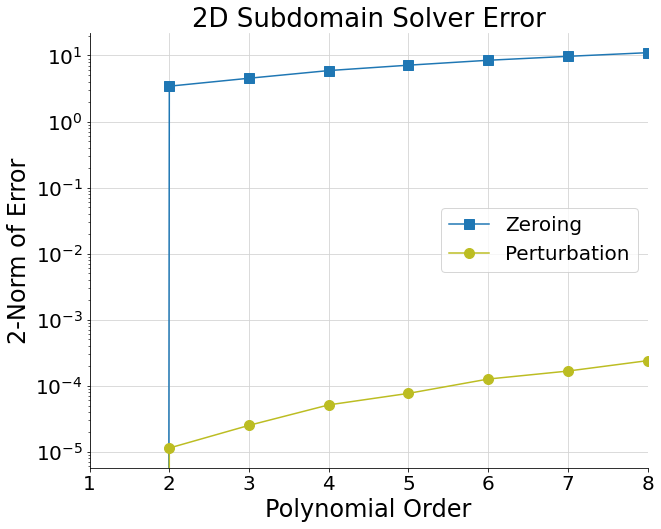
\includegraphics[width=0.48\textwidth]{../img/subdomainError2D}\label{fig:subdomain_pseudoinverse_2d}}
  \hfill
  \subfloat[2D Subdomain Error]{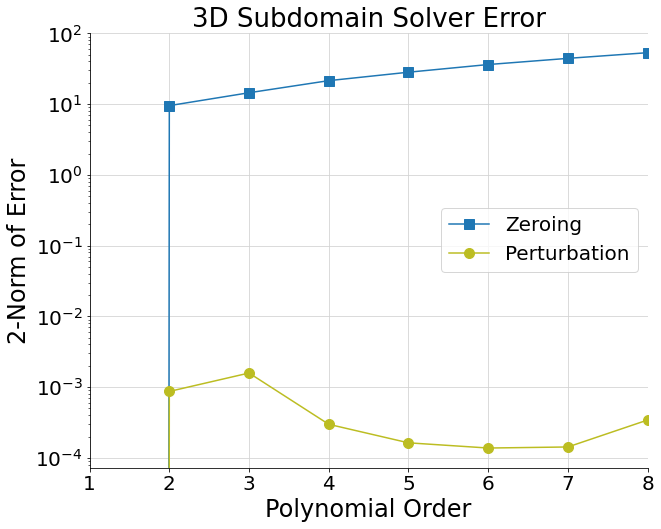
\includegraphics[width=0.48\textwidth]{../img/subdomainError3D}\label{fig:subdomain_pseudoinverse_3d}}
  \caption{Subdomain Pseudo-inverse Comparison}
  \label{fig:subdomain_pseudoinverse}
\end{figure}

In Figure \ref{fig:subdomain_pseudoinverse}, we compare these two methods of forming a pesudo-inverse of the Laplacian on a reference element.
We attempt to invert the action of the Laplacian, $\mathbf{K} \mathbf{u}$, on a two and three-dimensional reference element with polynomial bases of varying order with Dirichlet boundary conditions on the primal vertices.
The values in the vector $\mathbf{u}$ are given by $f \left( \mathbf{x} \right) = - \sum_d \left( \mathbf{x}_d + 1 \right) \left( \mathbf{x}_d - 1 \right)$.

Figure \ref{fig:subdomain_pseudoinverse_2d} shows the difference in the $L^2$ norm of the error between forming the pseudo-inverse by taking the reciprocal of the non-zero values in the eigenvalues of the two-dimensional Laplacian and using the true inverse of the two-dimensional Laplacian with a perturbation given by $\boldsymbol{\mathcal{K}} = \mathbf{K} + 1^{-6} \mathbf{I}$.
Figure \ref{fig:subdomain_pseudoinverse_3d} shows the difference in the $L^2$ norm of the error between forming the pseudo-inverse by taking the reciprocal of the non-zero values in the eigenvalues of the three-dimensional Laplacian and using the true inverse of the three-dimensional Laplacian with a perturbation given by $\boldsymbol{\mathcal{K}} = \mathbf{K} + 1^{-8} \mathbf{I}$.
In both figures we see that forming the pseudo-inverse on the reference element by computing the true inverse of the perturbed Laplacian results in a more accurate subdomain inverse.

For separable problems that can be expressed as a linear combination of the mass and Laplacian matrices
\begin{equation}
\mathbf{A} = a \mathbf{M} + b \mathbf{K}
\end{equation}
the FDM can provide a fast direct solver if the problem is invertible or a fast approximate inverse if the problem is not.
\begin{equation}
\mathbf{A}^{-1} = \mathbf{S}^T \left( a \mathbf{I} + b \boldsymbol{\Lambda} \right)^{-1} \mathbf{S}
\label{eq:fdminverse}
\end{equation}

Note that the inverse given in Equation \ref{eq:fdminverse} is similar to the element operator form given in Equation \ref{eq:localoperator}.
If we have an element operator defined by ${\color{burgundy}\mathbf{A}}^e = a \mathbf{M} + b \mathbf{K}$, then we can define an element inverse operator as ${\color{burgundy}\mathbf{A}}^{e, -1} = {\color{blue(ncs)}\mathbf{B}}^T {\color{applegreen}\mathbf{D}} {\color{blue(ncs)}\mathbf{B}}$, with ${\color{blue(ncs)}\mathbf{B}} = \mathbf{S}$ and ${\color{applegreen}\mathbf{D}} = \left( a \mathbf{I} + b \boldsymbol{\Lambda} \right)^{-1}$.
If the operator is not invertible, such as the Laplacian on a single element subdomain, we can still compute the approximate element inverse in this form.

This discussion of the FDM has, thus far, neglected the effects of irregular geometry, varying coefficients, or more complex PDEs.
These effects destroy the separability of this problem and the FDM cannot be used as fast direct solver for these problems.
However, as discussed by Li and Widlund in \cite{li2007use}, an inexact subdomain solver is adequate when BDDC is used as a preconditioner.

Couzy in \cite{couzy1995spectral} and Fischer, Miller, and Tofu in \cite{fischer2000overlapping} presented a simple modification to the FDM to address irregular geometry.
In their work, the Poisson problem is defined on a regular parallelepiped with average dimensions in each coordinate direction that match the finite element with the more complex geometry.
Here we present a further generalization which allows us to create an approximate FDM subdomain solver, ${\color{burgundy}\mathbf{A}}_{\text{r}, \text{r}}^{-1}$.

First we compute the simultaneous diagonalization of the mass and perturbed Laplacian matrices, as given in Equation \ref{eq:fdminverse}.
The eigenvectors from the diagonalization become the basis interpolation operator for our approximate FDM subdomain solver.
Our goal is to provide an adequate diagonal operator ${\color{applegreen}\mathbf{D}}$ to create a sufficiently accurate approximate subdomain inverse.

Recall that the operator representing the application of the weak form at quadrature points, ${\color{applegreen}\mathbf{D}}$, is block diagonal with the action of the PDE on each quadrature point independent from the other quadrature points.
We compute an average element coefficient by dividing out the quadrature weight for each entry in ${\color{applegreen}\mathbf{D}}$ and averaging the resulting matrix entries.

\begin{definition}[Average Element Coefficient]\label{def:averageelementcoefficient}
We denote the diagonal block for quadrature point $i$ by ${\color{applegreen}\mathbf{D}}_i$ and compute an \textit{average element coefficient} as
\begin{equation}
\bar{k}^e = \sum_{i \in 1, ..., q^d} \sum_{j, k \in 1, ..., m} \frac{\left( {\color{applegreen}\mathbf{D}}_{i} \right)_{j, k}}{\text{nnz} \left( {\color{applegreen}\mathbf{D}} \right) \mathbf{W}_i}
\end{equation}
where $\text{nnz} \left( {\color{applegreen}\mathbf{D}} \right)$ is the number of nonzero entries in the sparse matrix representation of the diagonal operator, $\mathbf{W}_i$ is the quadrature weight for quadrature point $i$, and $m$ is the number of evaluation modes for the operator, $1$ for interpolated values, $d$ for derivatives in $d$ dimensions, and $1 + d$ for a weak form with both interpolated values and derivatives at quadrature points.
\end{definition}

This average element coefficient is used to compute the approximate subdomain inverse diagonal
\begin{equation}
\begin{array}{c c}
\boldsymbol{\Lambda}^e = \bar{k}^e \boldsymbol{\Lambda},  &  \boldsymbol{\Lambda}^{e, -1} = \frac{1}{\bar{k}^e} \boldsymbol{\Lambda}^{-1},
\end{array}
\end{equation}
where the value of $\mathbf{\Lambda}$ is given by
\begin{equation}
\begin{array}{c}
\boldsymbol{\Lambda}_N      = \left( I \otimes I \otimes I \right)  \\
\boldsymbol{\Lambda}_D      = \left( \Lambda \otimes I \otimes I\right) + \left( I \otimes \Lambda \otimes I\right) + \left( I \otimes I \otimes \Lambda \right)  \\
\boldsymbol{\Lambda}_{N, D} = \boldsymbol{\Lambda}_N + \boldsymbol{\Lambda}_D  \\
\end{array}
\end{equation}
based upon if the diagonal operator ${\color{applegreen}\mathbf{D}}$ has interpolated values, derivatives, or both, respectively, at quadrature points.

We have an approximate FDM inverse for the entire subdomain, ${\color{burgundy}\mathbf{A}}^{e, +} = {\color{blue(ncs)}\mathbf{B}}^T {\color{applegreen}\mathbf{D}} {\color{blue(ncs)}\mathbf{B}}$, but we need a subdomain solver for only the broken space, ${\color{burgundy}\mathbf{A}}^{-1, e}_{\text{r}, \text{r}}$.
We form a saddle point problem to constrain the subdomain vertex nodes and form a Dirichlet problem from the full subdomain Neumann problem.
The subdomain problem is therefore given by

\begin{equation}
{\color{burgundy}\mathbf{A}}^e_{\text{r}, \text{r}} = \boldsymbol{\mathcal{R}}^T
\left[ \begin{array}{c c}
{\color{burgundy}\mathbf{A}}^e  &  \boldsymbol{\mathcal{V}}^T  \\
\boldsymbol{\mathcal{V}}        &  \mathbf{0}                  \\
\end{array} \right]
\boldsymbol{\mathcal{R}},
\end{equation}
where $\boldsymbol{\mathcal{R}}$ is an injection operator from the broken element space to the full element augmented with duplicate primal nodes to constrain and $\boldsymbol{\mathcal{V}}$ is the primal restriction operator, which restricts to the duplicated primal vertices from the full broken space.

\begin{definition}[Fast Diagonalization Method Approximate Subdomain Solver]
The Fast Diagonalization Method approximate inverse subdomain solver is given by the direct sum of element subdomain solvers of the form
\begin{equation}
{\color{burgundy}\mathbf{A}}^{e, -1}_{\text{r}, \text{r}} \approx {\color{burgundy}\mathbf{A}}^{e, +}_{\text{r}, \text{r}} = \boldsymbol{\mathcal{R}}^T
\left[ \begin{array}{c c}
{\color{burgundy}\mathbf{A}}^{e, +}  &  -{\color{burgundy}\mathbf{A}}^{e, +} \boldsymbol{\mathcal{V}}^T \mathbf{S}^{-1}  \\
\mathbf{0}                           &  \mathbf{S}^{-1}                                                     \\
\end{array} \right]
\left[ \begin{array}{c c}
\mathbf{I}                                                      &  \mathbf{0}  \\
- \boldsymbol{\mathcal{V}} {\color{burgundy}\mathbf{A}}^{e, +}  &  \mathbf{I}  \\
\end{array} \right]
\boldsymbol{\mathcal{R}},
\end{equation}
where $\mathbf{S} = - \boldsymbol{\mathcal{V}} {\color{burgundy}\mathbf{A}}^{e, +} \boldsymbol{\mathcal{V}}^T$, $\boldsymbol{\mathcal{R}}$ is an injection operator from the duplicate primal vertices to the full element, and $\boldsymbol{\mathcal{V}}$ is the primal restriction operator, which restricts to the primal vertices from the full element.
The approximate inverse for each subdomain is given by
\begin{equation}
{\color{burgundy}\mathbf{A}}^{e, +} = {\color{blue(ncs)}\mathbf{B}}^T {\color{applegreen}\mathbf{D}} {\color{blue(ncs)}\mathbf{B}},
\end{equation}
where ${\color{blue(ncs)}\mathbf{B}}$ is a basis interpolating to the eigenspace of the simultaneous diagonalization of the mass and perturbed Laplacian matrices $\mathbf{M} = \mathbf{N}^T \mathbf{W} \mathbf{N}$ and $\boldsymbol{\mathcal{K}} = \mathbf{D}^T \mathbf{W} \mathbf{D} + \epsilon \mathbf{I}$.
${\color{applegreen}\mathbf{D}}$ is computed from the eigenvalues of this diagonalization and the average element coefficient value, from Definition \ref{def:averageelementcoefficient},
\begin{equation}
\begin{array}{c c}
\boldsymbol{\Lambda}^e = \bar{k}^e \boldsymbol{\Lambda},  &  \boldsymbol{\Lambda}^{e, -1} = \frac{1}{\bar{k}^e} \boldsymbol{\Lambda}^{-1},
\end{array}
\end{equation}
where the value of $\mathbf{\Lambda}$ is given by
\begin{equation}
\begin{array}{c}
\boldsymbol{\Lambda}_N      = \left( I \otimes I \otimes I \right)  \\
\boldsymbol{\Lambda}_D      = \left( \Lambda \otimes I \otimes I\right) + \left( I \otimes \Lambda \otimes I\right) + \left( I \otimes I \otimes \Lambda \right)  \\
\boldsymbol{\Lambda}_{N, D} = \boldsymbol{\Lambda}_N + \boldsymbol{\Lambda}_D  \\
\end{array}
\end{equation}
based upon if the weak form for operator ${\color{burgundy}\mathbf{A}}^e$ has interpolated values, derivatives, or both, respectively, at quadrature points.
\end{definition}

The subdomain interior solver can also be computed from this fast diagonalization of the element matrix.
Reusing the fast diagonalization for both the subdomain solver and subdomain interior eliminates the higher setup cost of the Dirichlet BDDC compared to the lumped BDDC.

\begin{definition}[Fast Diagonalization Method Approximate Subdomain Interior Solver]
The Fast Diagonalization Method approximate inverse subdomain interior solver is given by the direct sum of element subdomain solvers of the form
\begin{equation}
{\color{burgundy}\mathbf{A}}^{e, -1}_{\text{r}, \text{r}} \approx {\color{burgundy}\mathbf{A}}^{e, +}_{\text{r}, \text{r}} = \boldsymbol{\mathcal{R}}^T
\left[ \begin{array}{c c}
{\color{burgundy}\mathbf{A}}^{e, +}  &  -{\color{burgundy}\mathbf{A}}^{e, +} \boldsymbol{\mathcal{V}}^T \mathbf{S}^{-1}  \\
\mathbf{0}                           &  \mathbf{S}^{-1}                                                     \\
\end{array} \right]
\left[ \begin{array}{c c}
\mathbf{I}                                                      &  \mathbf{0}  \\
- \boldsymbol{\mathcal{V}} {\color{burgundy}\mathbf{A}}^{e, +}  &  \mathbf{I}  \\
\end{array} \right]
\boldsymbol{\mathcal{R}},
\end{equation}
where $\mathbf{S} = - \boldsymbol{\mathcal{V}} {\color{burgundy}\mathbf{A}}^{e, +} \boldsymbol{\mathcal{V}}^T$, $\boldsymbol{\mathcal{R}}$ is an injection operator from the duplicate interface vertices to the full element, and $\boldsymbol{\mathcal{V}}$ is the interface restriction operator, which restricts to the interface vertices from the element.
The approximate inverse for each subdomain is given by
\begin{equation}
{\color{burgundy}\mathbf{A}}^{e, +} = {\color{blue(ncs)}\mathbf{B}}^T {\color{applegreen}\mathbf{D}} {\color{blue(ncs)}\mathbf{B}},
\end{equation}
where ${\color{blue(ncs)}\mathbf{B}}$ is a basis interpolating to the eigenspace of the simultaneous diagonalization of the mass and perturbed Laplacian matrices $\mathbf{M} = \mathbf{N}^T \mathbf{W} \mathbf{N}$ and $\boldsymbol{\mathcal{K}} = \mathbf{D}^T \mathbf{W} \mathbf{D} + \epsilon \mathbf{I}$.
${\color{applegreen}\mathbf{D}}$ is computed from the eigenvalues of this diagonalization and the average element coefficient value, from Definition \ref{def:averageelementcoefficient},
\begin{equation}
\begin{array}{c c}
\boldsymbol{\Lambda}^e = \bar{k}^e \boldsymbol{\Lambda},  &  \boldsymbol{\Lambda}^{e, -1} = \frac{1}{\bar{k}^e} \boldsymbol{\Lambda}^{-1},
\end{array}
\end{equation}
where the value of $\mathbf{\Lambda}$ is given by
\begin{equation}
\begin{array}{c}
\boldsymbol{\Lambda}_N      = \left( I \otimes I \otimes I \right)  \\
\boldsymbol{\Lambda}_D      = \left( \Lambda \otimes I \otimes I\right) + \left( I \otimes \Lambda \otimes I\right) + \left( I \otimes I \otimes \Lambda \right)  \\
\boldsymbol{\Lambda}_{N, D} = \boldsymbol{\Lambda}_N + \boldsymbol{\Lambda}_D  \\
\end{array}
\end{equation}
based upon if the weak form for operator ${\color{burgundy}\mathbf{A}}^e$ has interpolated values, derivatives, or both, respectively, at quadrature points.
\end{definition}